\documentclass[conference]{IEEEtran}
\IEEEoverridecommandlockouts
% The preceding line is only needed to identify funding in the first footnote. If that is unneeded, please comment it out.
\usepackage{cite}
\usepackage{amsmath,amssymb,amsfonts}
\usepackage{algorithmic}
\usepackage{graphicx}
\usepackage{textcomp}
\usepackage{xcolor}
\usepackage{gensymb}
\usepackage{float}

% Python shit..
% Default fixed font does not support bold face
\DeclareFixedFont{\ttb}{T1}{txtt}{bx}{n}{12} % for bold
\DeclareFixedFont{\ttm}{T1}{txtt}{m}{n}{12}  % for normal

% Custom colors
\usepackage{color}
\definecolor{deepblue}{rgb}{0,0,0.5}
\definecolor{deepred}{rgb}{0.6,0,0}
\definecolor{deepgreen}{rgb}{0,0.5,0}

\usepackage{listings}

% Python style for highlighting
\newcommand\pythonstyle{\lstset{
breaklines=true,
postbreak=\mbox{\textcolor{red}{$\hookrightarrow$}\space},
language=Python,
basicstyle=\ttm,
otherkeywords={self},             % Add keywords here
keywordstyle=\ttb\color{deepblue},
emph={MyClass,__init__},          % Custom highlighting
emphstyle=\ttb\color{deepred},    % Custom highlighting style
stringstyle=\color{deepgreen},
frame=tb,                         % Any extra options here
showstringspaces=false            % 
}}
% Python environment
\lstnewenvironment{python}[1][]
{
\pythonstyle
\lstset{#1}
}
{}

% Python for external files
\newcommand\pythonexternal[2][]{{
\pythonstyle
\lstinputlisting[#1]{#2}}}

% Python for inline
\newcommand\pythoninline[1]{{\pythonstyle\lstinline!#1!}}


\usepackage[center]{caption}
\def\BibTeX{{\rm B\kern-.05em{\sc i\kern-.025em b}\kern-.08em
    T\kern-.1667em\lower.7ex\hbox{E}\kern-.125emX}}
\begin{document}

\title{Machine Perception 2020\\
{\footnotesize \textsuperscript{Curtin University - Perth}}
}

\author{\IEEEauthorblockN{Jonathan Wright}
\IEEEauthorblockA{\textit{Curtin University} \\
\textit{Computer Science Student}\\
Perth, WA \\
19779085@student.curtin.edu.au}}

\maketitle
\begin{figure}[!htbp]
    \centerline{{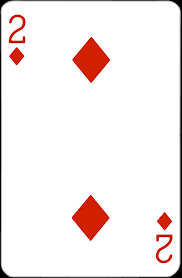
\includegraphics[width=20mm, scale=0.5]{./figures/diamond2.png}}
    {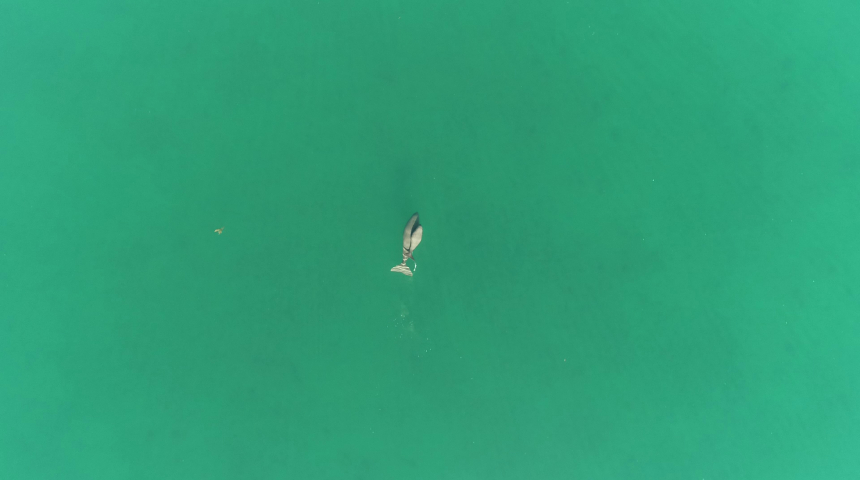
\includegraphics[width=50mm, scale=0.5]{./figures/Dugong.jpg}}}
    \caption{Source Images:\\*
    1 - Red Diamond Playing Card \\*
    2 - Dugong, Calf with Seaweed.}
    \label{fig}
\end{figure}
\begin{abstract}
This paper will explore questions asked by the Machine Perception 2020 Assignment 1 Paper, this expands to
1 - Image Histograms, Harris Corner and SIFT Key variance/invariance.
2 - LBP, HOG and SIFT Feature Extraction.
3 - Object Extraction using CCL on Figures 1 and 2.
4 - Image Segmentation on Figures 1 and 2 using K-Means and different colorspaces.
\end{abstract}
\section{Task One}
\subsection{Generated Images}
For this section I have generated images of various rotations: (180\degree, 45\degree, -45\degree, 90\degree, -90\degree).\\*
I have also generated images of various scales: (100\%, 50\%, 25\%, 50\% Height 100\% Width, 50\% Width 100\% Height)
\subsection{Image Histograms}
\begin{figure}[H]
    \centerline{
        {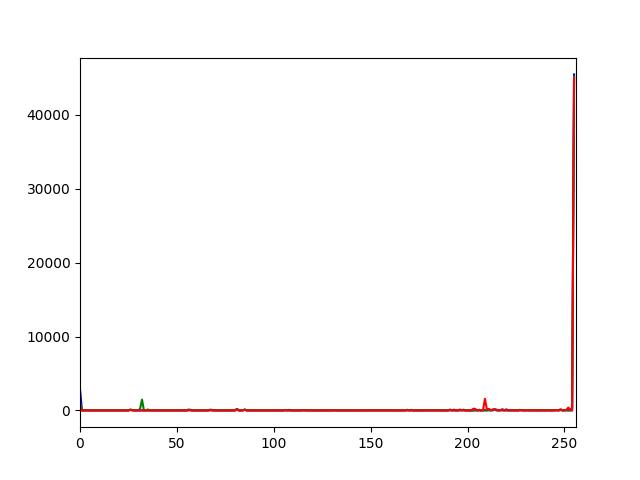
\includegraphics[width=20mm, scale=0.5]{./figures/RotationHists/diamondneutral Hist.png}}
        {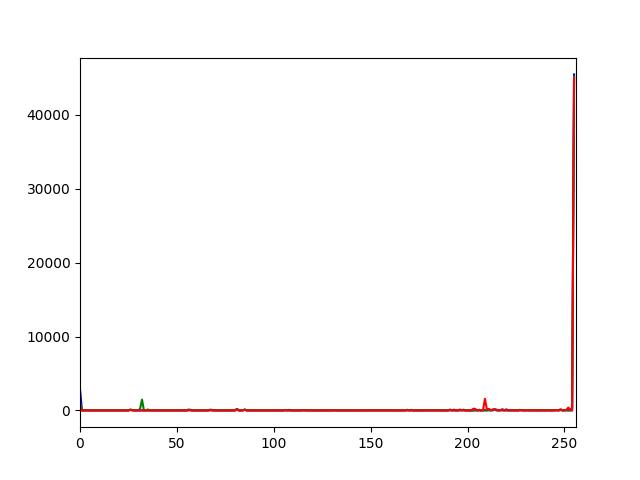
\includegraphics[width=20mm, scale=0.5]{./figures/RotationHists/diamonddeg90 Hist.png}}
        {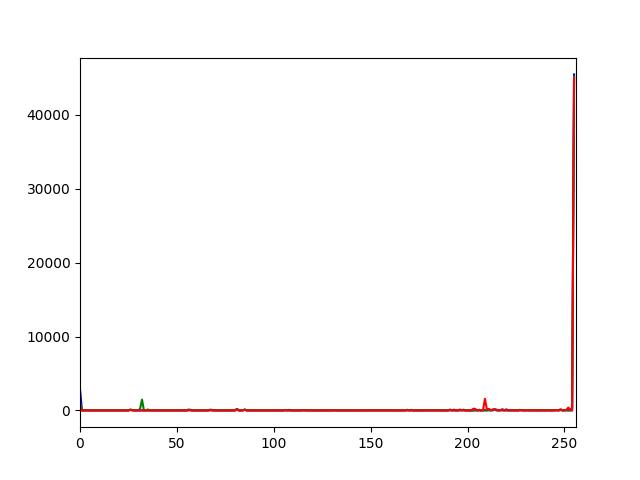
\includegraphics[width=20mm, scale=0.5]{./figures/RotationHists/diamonddegn90 Hist.png}}
    }
    \centerline{
        {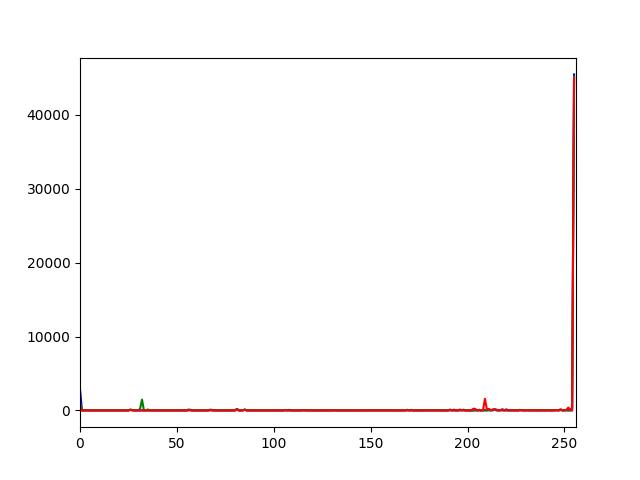
\includegraphics[width=20mm, scale=0.5]{./figures/RotationHists/diamondflipped Hist.png}}
        {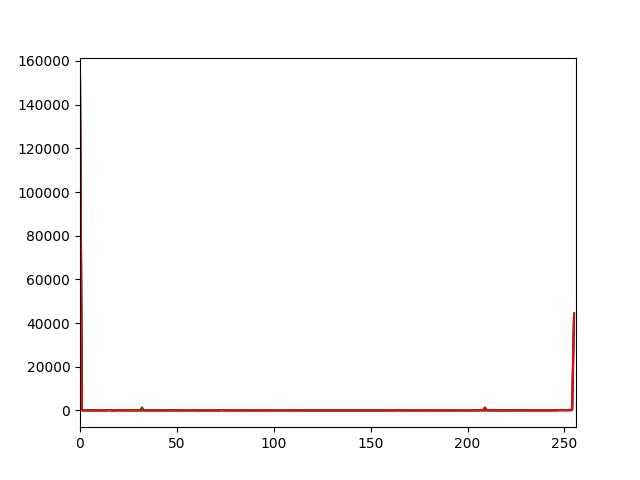
\includegraphics[width=20mm, scale=0.5]{./figures/RotationHists/diamonddeg45 Hist.png}}
        {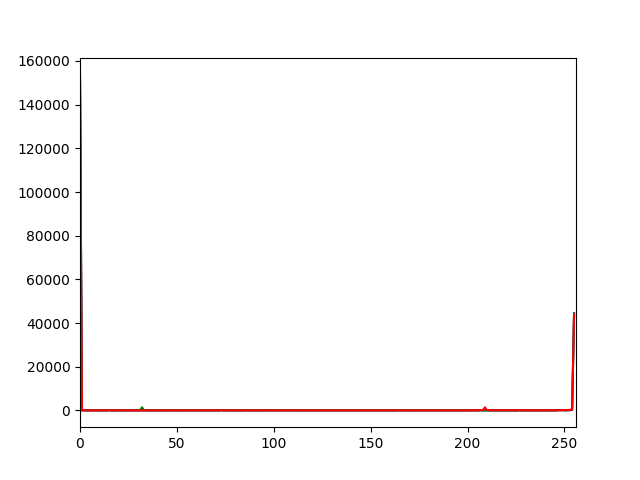
\includegraphics[width=20mm, scale=0.5]{./figures/RotationHists/diamonddegn45 Hist.png}}
    }
    \caption{Diamond Rotation Histograms: (Neutral, -90\degree, 90\degree, 180\degree, 45\degree and -45\degree\ NOTE: 45 Degrees will not be the same due to adding black)}
    \label{fig}
\end{figure}
\begin{figure}[H]
    \centerline{
        {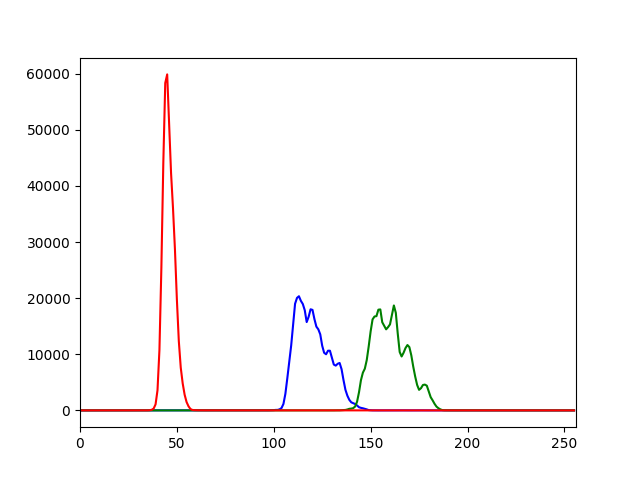
\includegraphics[width=20mm, scale=0.5]{./figures/RotationHists/Dugongneutral Hist.png}}
        {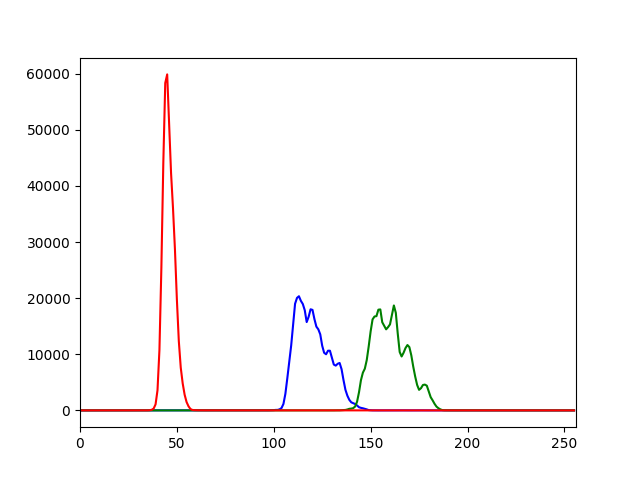
\includegraphics[width=20mm, scale=0.5]{./figures/RotationHists/Dugongdeg90 Hist.png}}
        {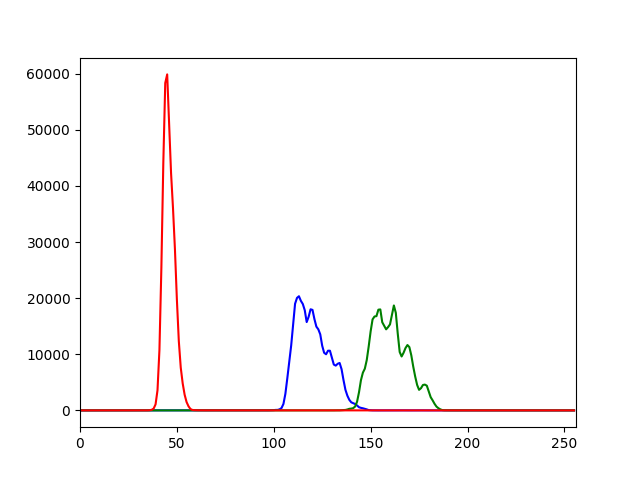
\includegraphics[width=20mm, scale=0.5]{./figures/RotationHists/Dugongdegn90 Hist.png}}
    }
    \centerline{
        {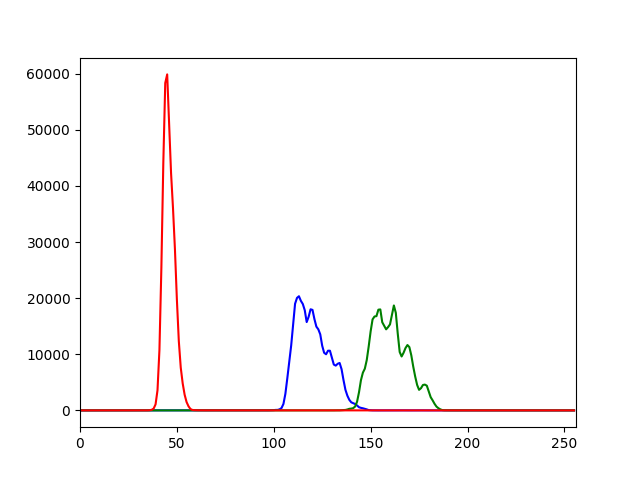
\includegraphics[width=20mm, scale=0.5]{./figures/RotationHists/Dugongflipped Hist.png}}
        {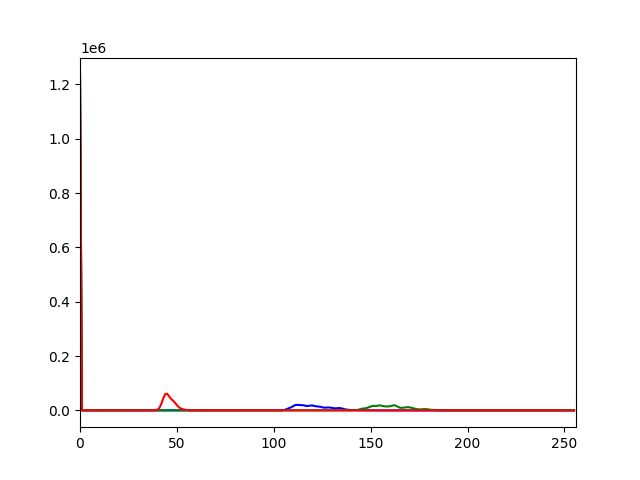
\includegraphics[width=20mm, scale=0.5]{./figures/RotationHists/Dugongdeg45 Hist.png}}
        {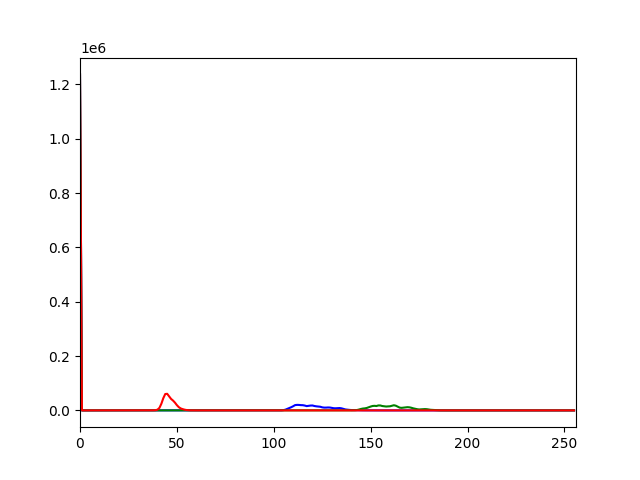
\includegraphics[width=20mm, scale=0.5]{./figures/RotationHists/Dugongdegn45 Hist.png}}
    }
    \caption{Dugong Rotation Histograms: (Neutral, -90\degree, 90\degree, 180\degree, 45\degree and -45\degree\ NOTE: 45 Degrees will not be the same due to adding black)}
    \label{fig}
\end{figure}
Rotation: \\*
Image Histograms are invariant to rotation, as you can see with my histograms they remain constant through rotations (90\degree, 180\degree, -90\degree, and 0\degree)
a important note to make is that while 45\degree and -45\degree are not the same as the rest, this is because I had to add additional black to the image to fit it on the canvas.\\
\begin{figure}[H]
    \centerline{
        {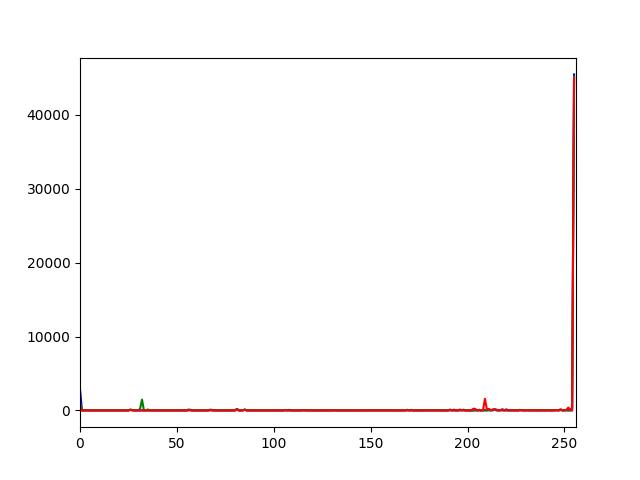
\includegraphics[width=20mm, scale=0.5]{./figures/ScalingHists/diamond.png}}
        {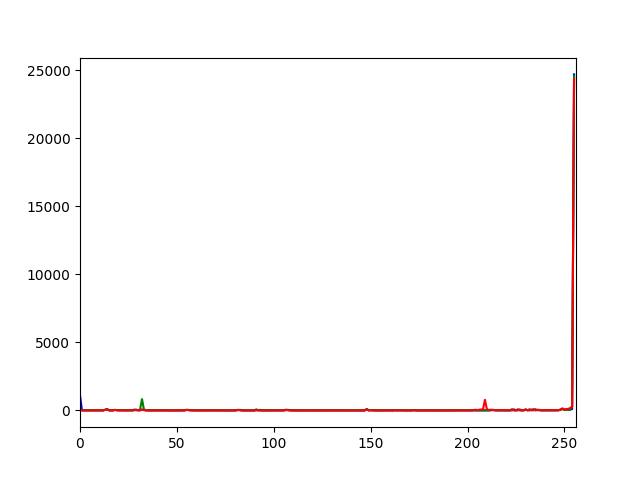
\includegraphics[width=20mm, scale=0.5]{./figures/ScalingHists/diamond75.png}}
        {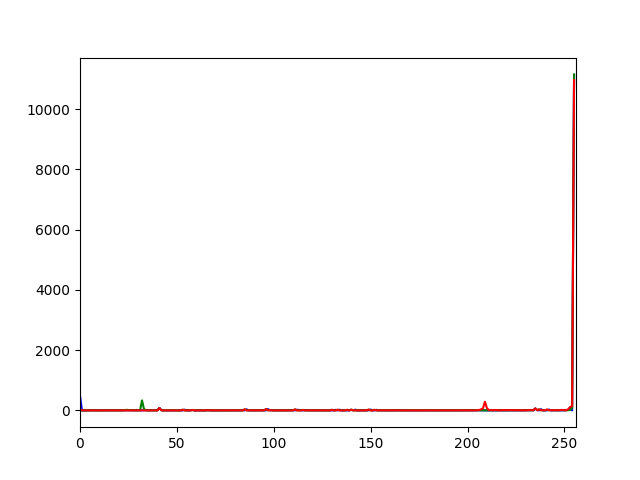
\includegraphics[width=20mm, scale=0.5]{./figures/ScalingHists/diamond50.png}}
    }
    \centerline{
        {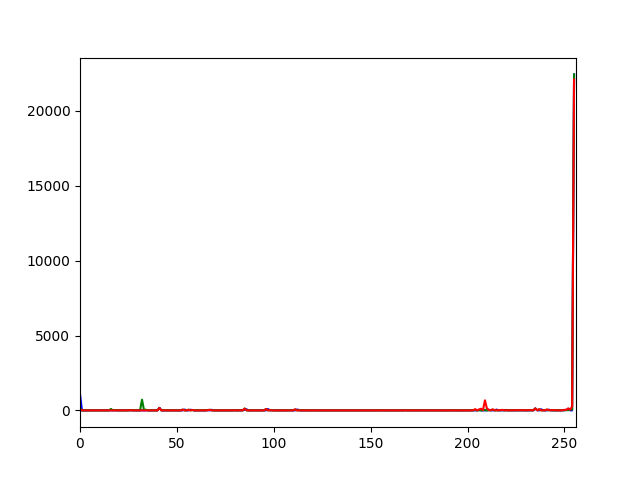
\includegraphics[width=20mm, scale=0.5]{./figures/ScalingHists/diamond50w.png}}
        {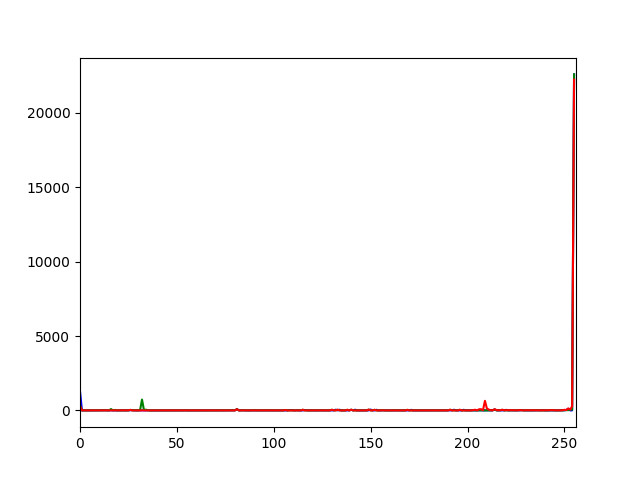
\includegraphics[width=20mm, scale=0.5]{./figures/ScalingHists/diamond50h.png}}
    }
    \caption{Diamond Scaling Histograms: (Neutral, 75\%, 50\%, 50\% width, 50\% height)}
    \label{fig}
\end{figure}
\begin{figure}[H]
    \centerline{
        {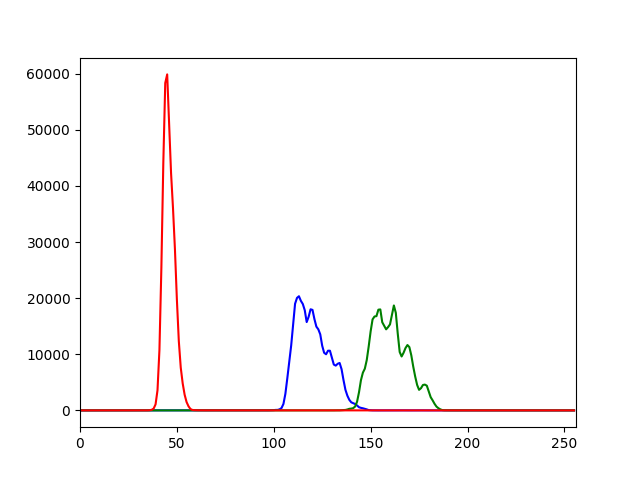
\includegraphics[width=20mm, scale=0.5]{./figures/ScalingHists/dugong.png}}
        {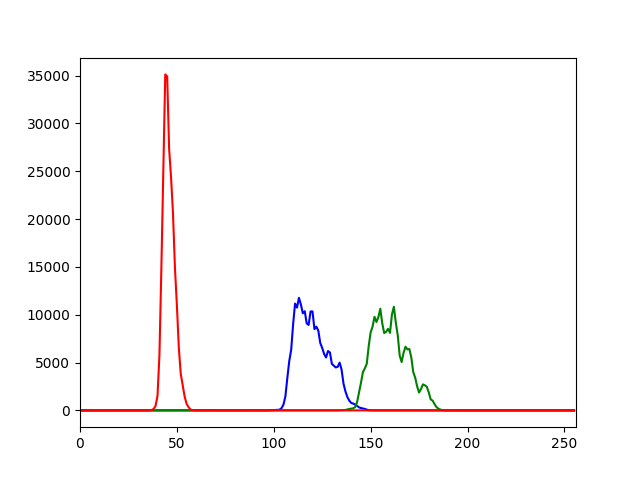
\includegraphics[width=20mm, scale=0.5]{./figures/ScalingHists/dugong75.png}}
        {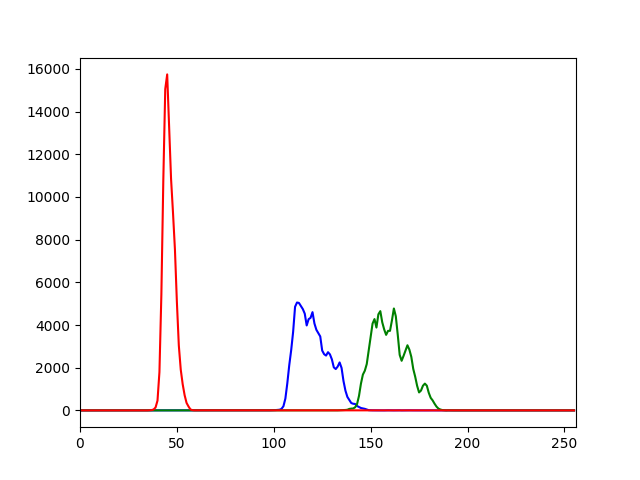
\includegraphics[width=20mm, scale=0.5]{./figures/ScalingHists/dugong50.png}}
    }
    \centerline{
        {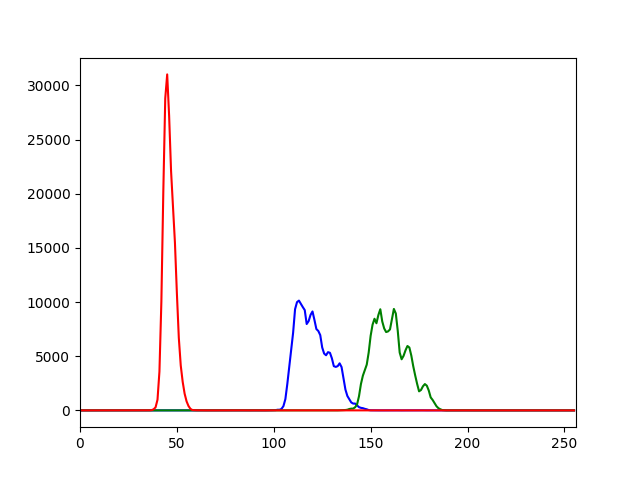
\includegraphics[width=20mm, scale=0.5]{./figures/ScalingHists/dugong50w.png}}
        {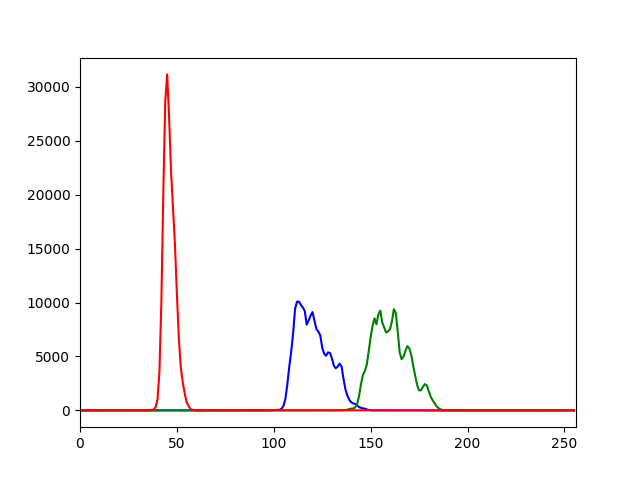
\includegraphics[width=20mm, scale=0.5]{./figures/ScalingHists/dugong50h.png}}
    }
    \caption{Dugong Scaling Histograms: (Neutral, 75\%, 50\%, 50\% width, 50\% height)}
    \label{fig}
\end{figure}
Scaling: \\*
Image Histograms are invariant to scaling, as you can see with my histograms they remain constant through scaling.
\subsection{Harris Corner Detectors}
\begin{figure}[H]
    \centerline{
        {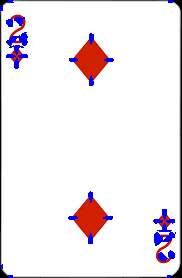
\includegraphics[width=10mm, scale=0.5]{./figures/Harris Corner/diamondNeutral Corners.png}}
        {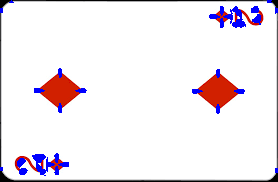
\includegraphics[width=20mm, scale=0.5]{./figures/Harris Corner/diamondDeg 90 Corners.png}}
        {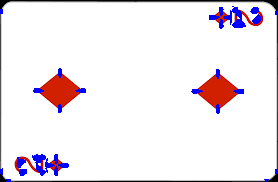
\includegraphics[width=20mm, scale=0.5]{./figures/Harris Corner/diamondDeg -90 Corners.png}}
    }
    \centerline{
        {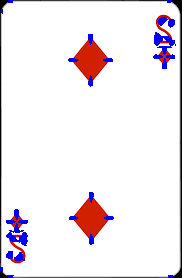
\includegraphics[width=15mm, scale=0.5]{./figures/Harris Corner/diamond180 Deg Corners.png}}
        {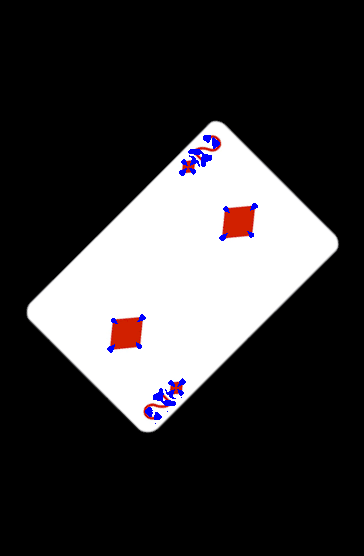
\includegraphics[width=15mm, scale=0.5]{./figures/Harris Corner/diamondDeg -45 Corners.png}}
        {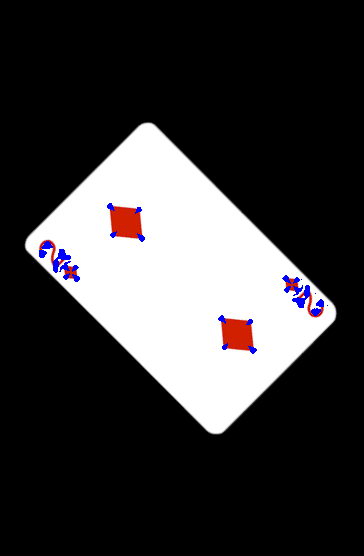
\includegraphics[width=15mm, scale=0.5]{./figures/Harris Corner/diamondDeg 45 Corners.png}}
    }
    \caption{Diamond Rotation Harris Corner Detections (Neutral, -90\degree, 90\degree, 180\degree, 45\degree and -45\degree)}
    \label{fig}
\end{figure}
\begin{figure}[H]
    \centerline{
        {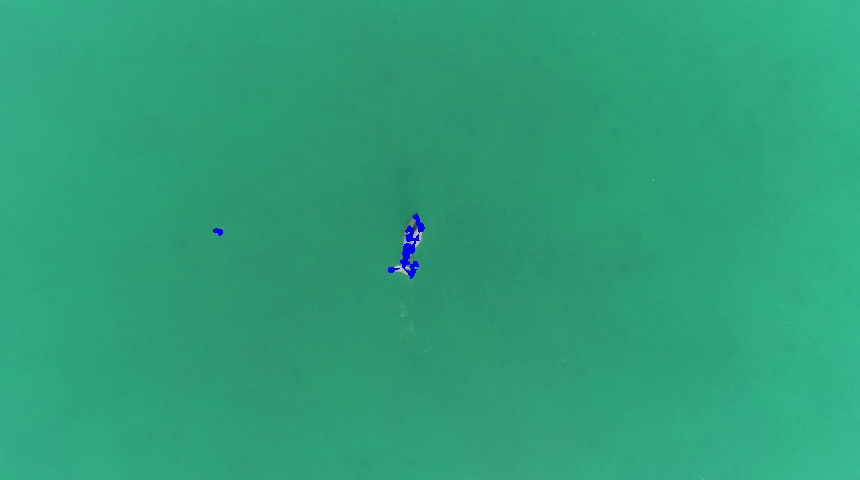
\includegraphics[width=40mm, scale=0.5]{./figures/Harris Corner/DugongNeutral Corners.png}}
        {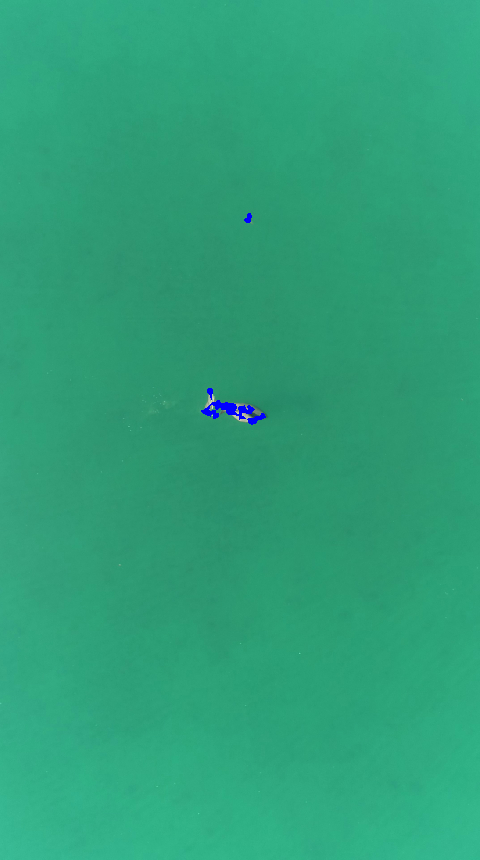
\includegraphics[width=20mm, scale=0.5]{./figures/Harris Corner/DugongDeg 90 Corners.png}}
        {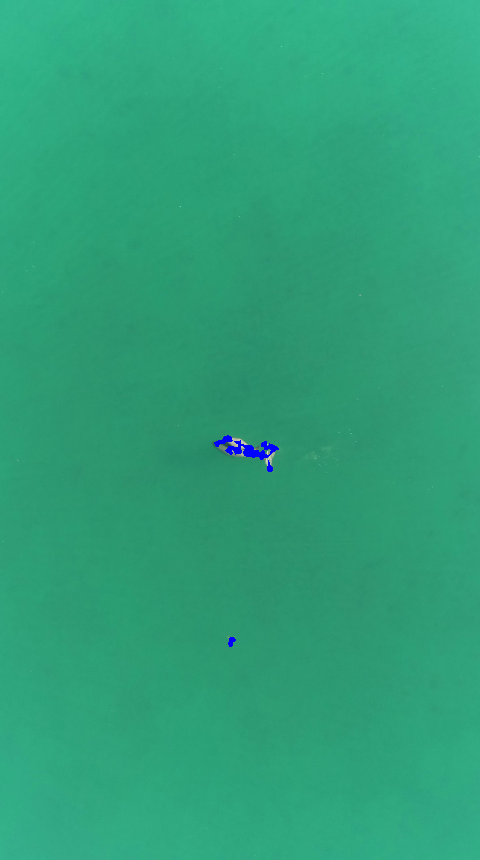
\includegraphics[width=20mm, scale=0.5]{./figures/Harris Corner/DugongDeg -90 Corners.png}}
    }
    \centerline{
        {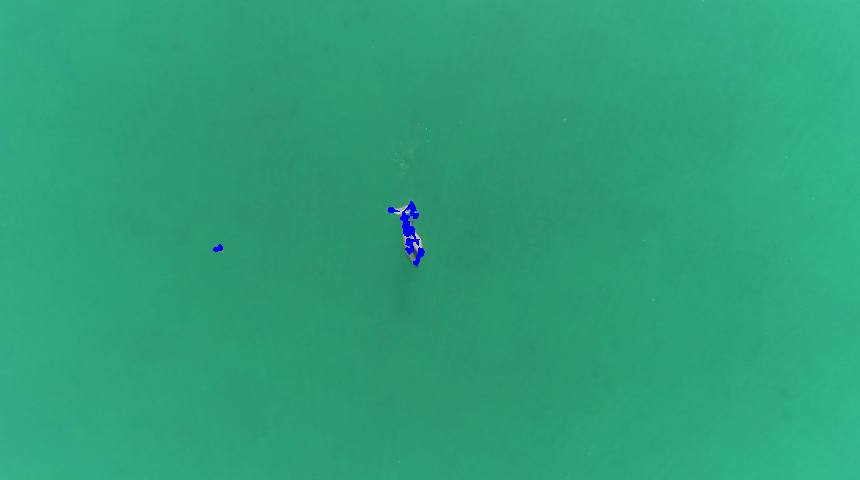
\includegraphics[width=30mm, scale=0.5]{./figures/Harris Corner/Dugong180 Deg Corners.png}}
        {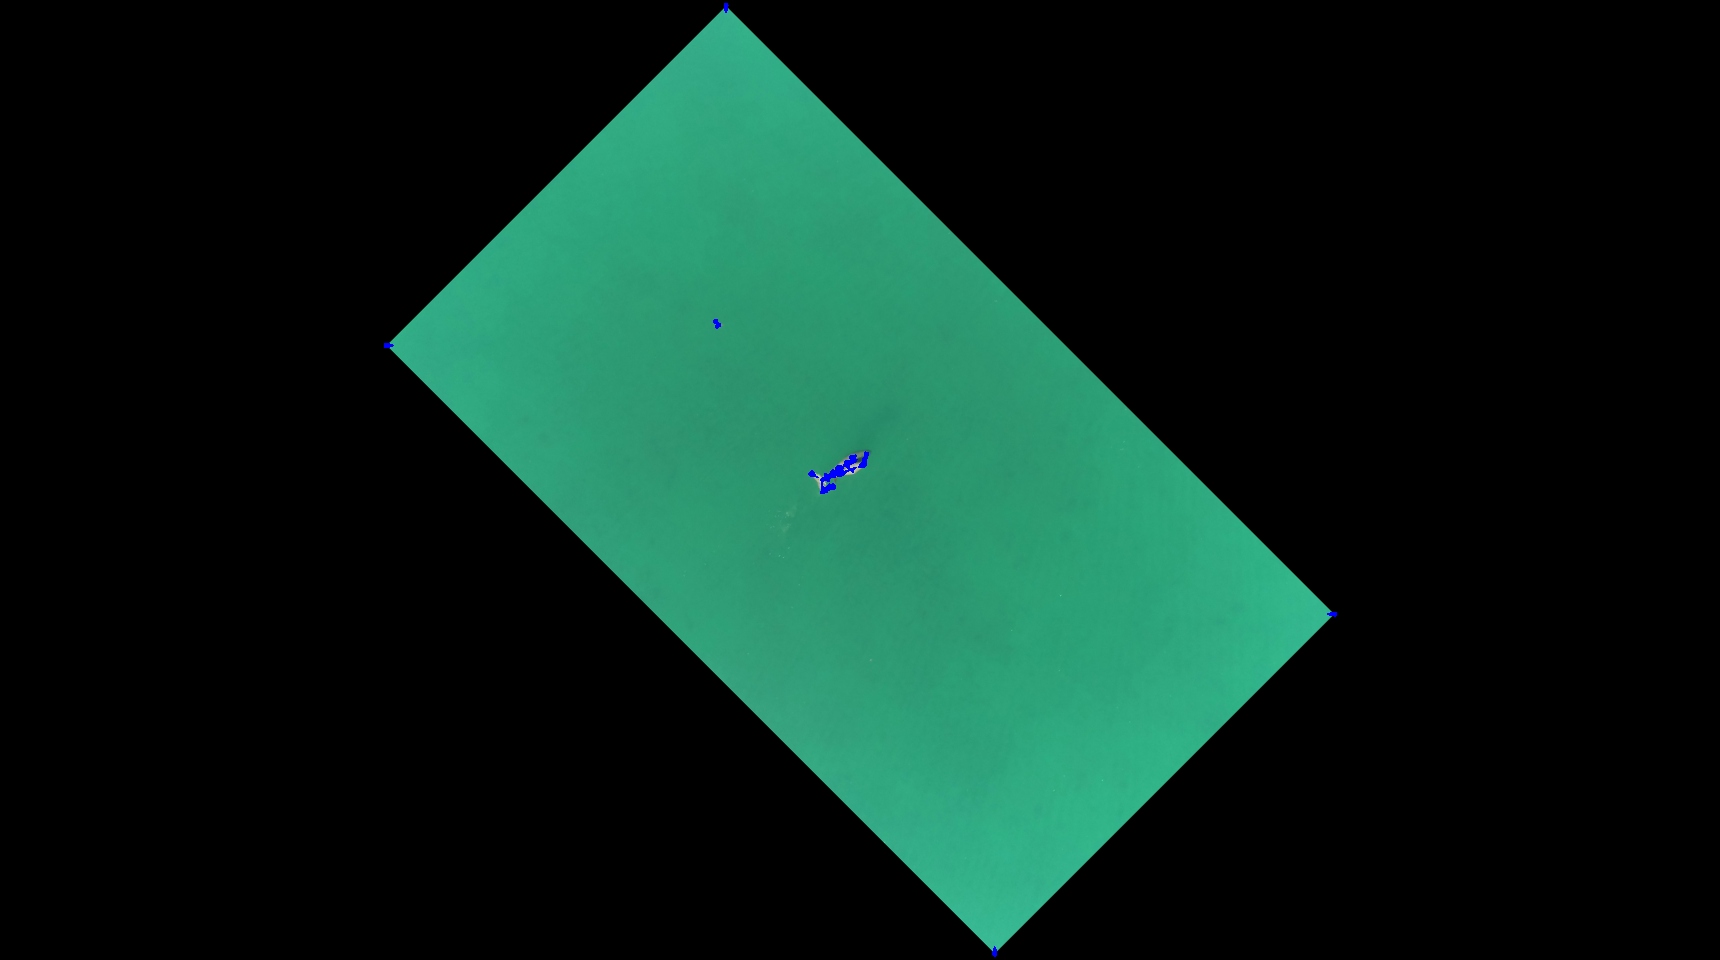
\includegraphics[width=30mm, scale=0.5]{./figures/Harris Corner/DugongDeg -45 Corners.png}}
        {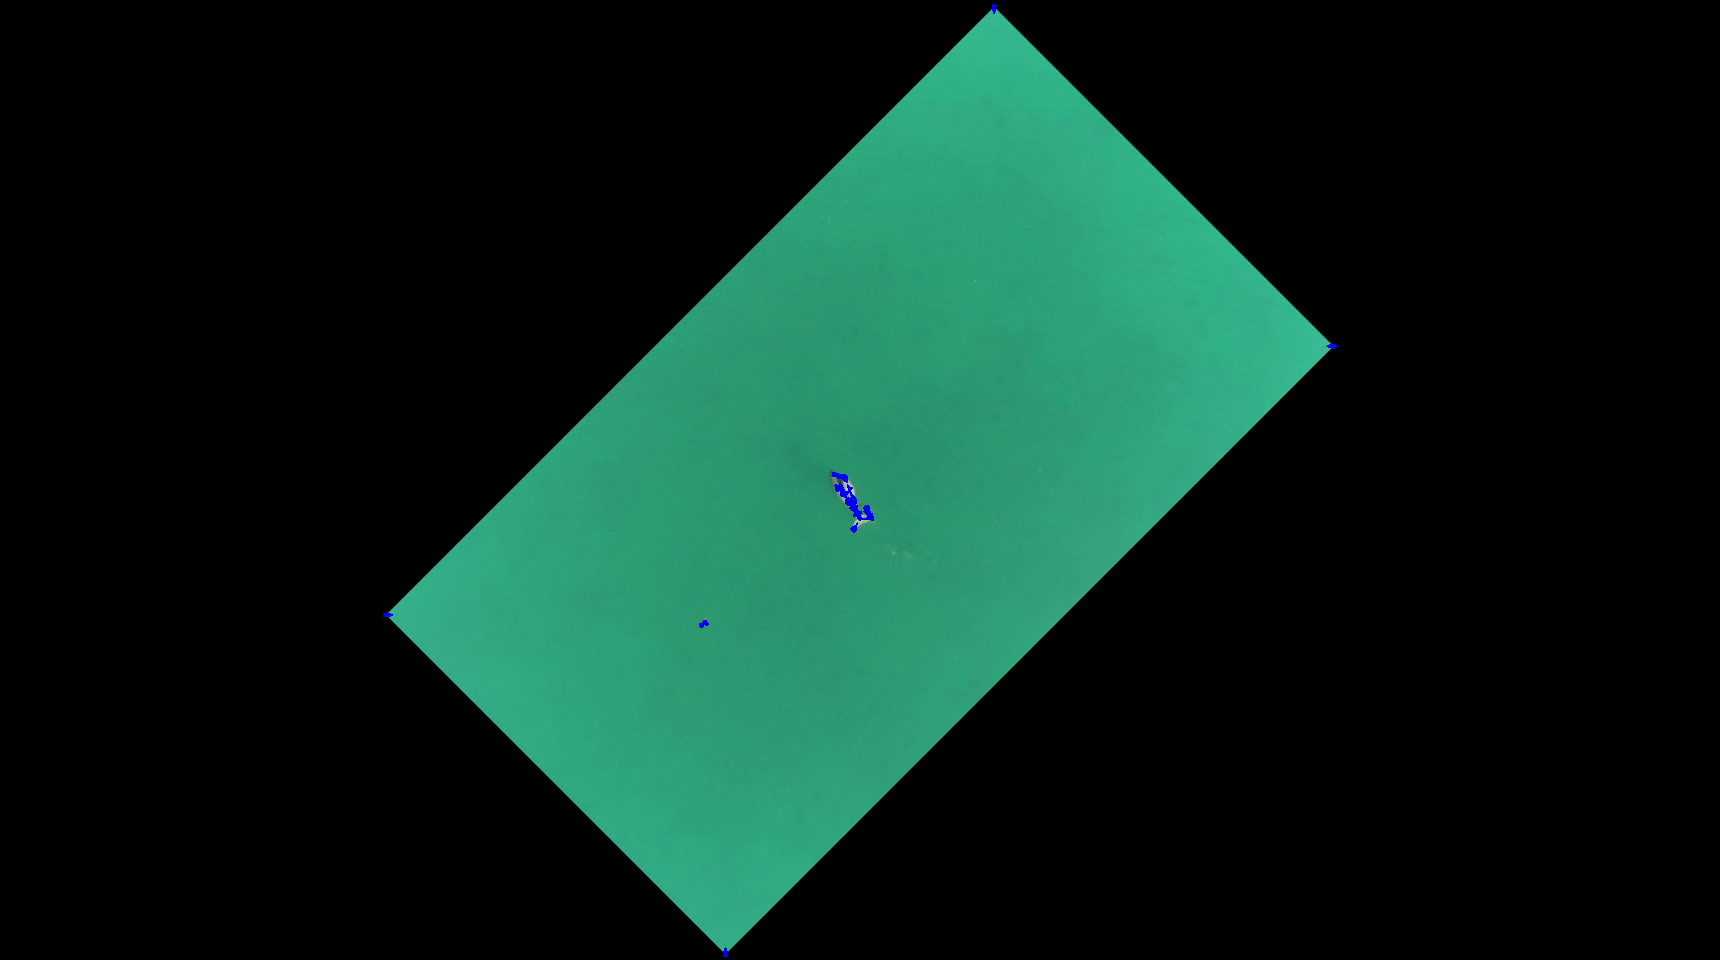
\includegraphics[width=30mm, scale=0.5]{./figures/Harris Corner/DugongDeg 45 Corners.png}}
    }
    \caption{Dugong Rotation Harris Corner Detections (Neutral, -90\degree, 90\degree, 180\degree, 45\degree and -45\degree)}
    \label{fig}
\end{figure}
Rotation: \\*
From the results above we can see that the same edges are being detected on all rotations with no variancy, as such we can conclude that Harris Corner Detection is rotation invariant.
\begin{figure}[H]
    \centerline{
        {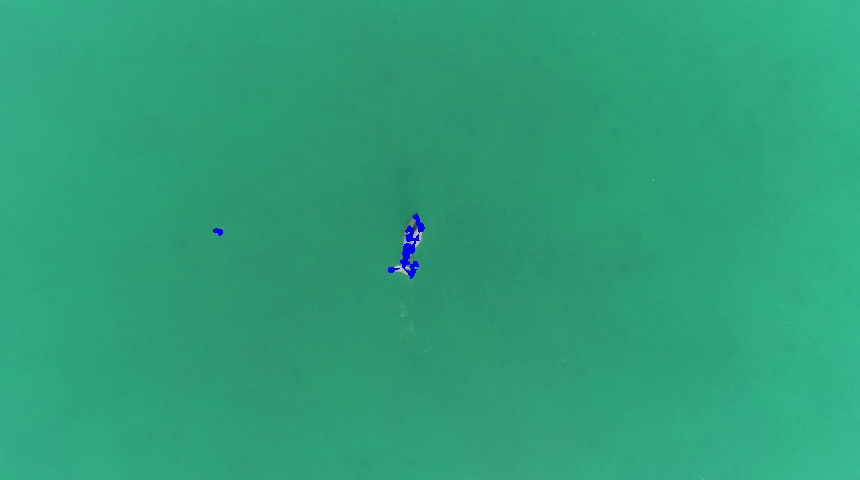
\includegraphics[width=20mm, scale=0.5]{./figures/Harris Corner/DugongNeutral Corners.png}}
        {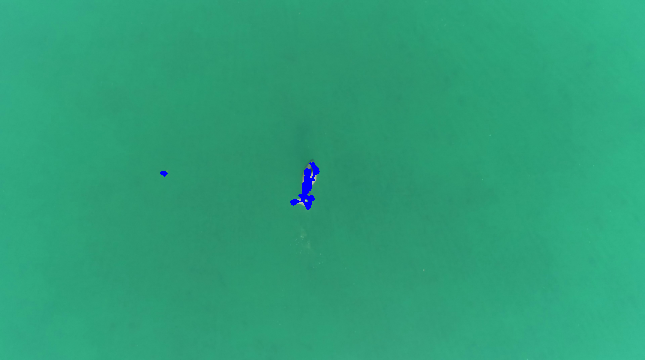
\includegraphics[width=20mm, scale=0.5]{./figures/Harris Corner/Dugong75 Corners.png}}
        {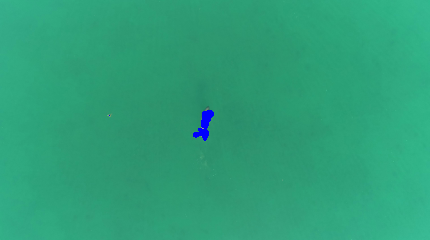
\includegraphics[width=20mm, scale=0.5]{./figures/Harris Corner/Dugong50 Corners.png}}
    }
    \centerline{
        {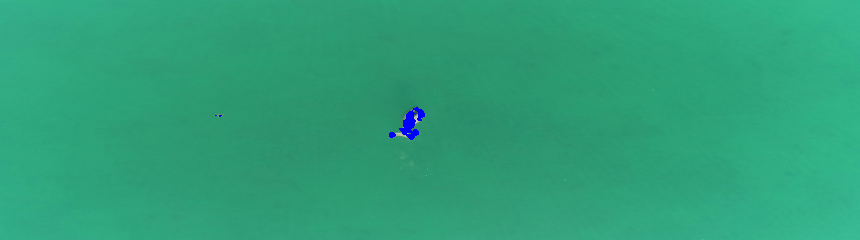
\includegraphics[width=40mm, scale=0.5]{./figures/Harris Corner/DugongheightReduced Corners.png}}
        {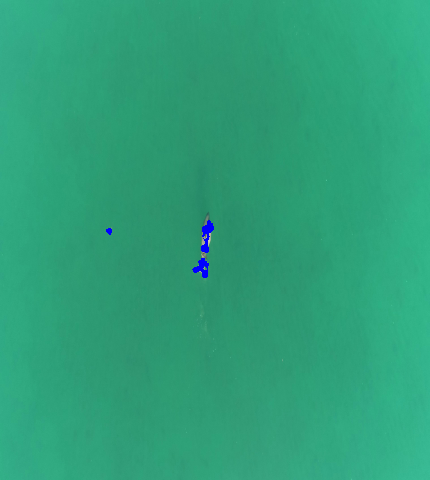
\includegraphics[width=20mm, scale=0.5]{./figures/Harris Corner/DugongwidthReduced Corners.png}}
    }
    \caption{Dugong Scaling Corner Detection: (Neutral, 75\%, 50\%, 50\% height, 50\% width)\\*
    While hard to see they are not the same!}
    \label{fig}
\end{figure}
\begin{figure}[H]
    \centerline{
        {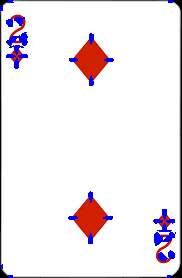
\includegraphics[width=20mm, scale=0.5]{./figures/Harris Corner/diamondNeutral Corners.png}}
        {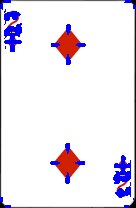
\includegraphics[width=20mm, scale=0.5]{./figures/Harris Corner/diamond75 Corners.png}}
        {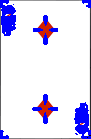
\includegraphics[width=20mm, scale=0.5]{./figures/Harris Corner/diamond50 Corners.png}}
    }
    \centerline{
        {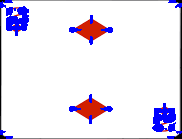
\includegraphics[width=20mm, scale=0.5]{./figures/Harris Corner/diamondheightReduced Corners.png}}
        {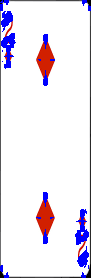
\includegraphics[width=10mm, scale=0.5]{./figures/Harris Corner/diamondwidthReduced Corners.png}}
    }
    \caption{Diamond Scaling Corner Detection: (Neutral, 75\%, 50\%, 50\% height, 50\% width)\\*
    While hard to see they are not the same!}
    \label{fig}
\end{figure}
Scaling:
From the results above I can conclude from visual inspection that Harris Corner Detection is scale variant, I conclude this by the fact that different edges are detected at different scales, sometimes the seaweed is not picked up (as in case 50\% height).
\\*
\subsection{SIFT Feature Detectors}
\begin{figure}[H]
    \centerline{
        {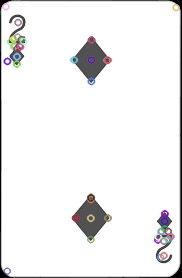
\includegraphics[width=20mm, scale=0.5]{./figures/SIFT/diamondNeutral SIFT.png}}
        {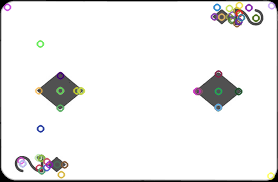
\includegraphics[width=20mm, scale=0.5]{./figures/SIFT/diamondDeg 90 SIFT.png}}
        {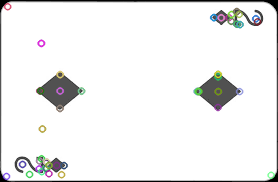
\includegraphics[width=20mm, scale=0.5]{./figures/SIFT/diamondDeg -90 SIFT.png}}
    }
    \centerline{
        {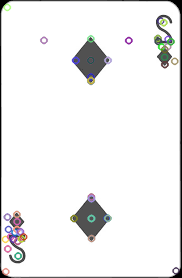
\includegraphics[width=20mm, scale=0.5]{./figures/SIFT/diamond180 Deg SIFT.png}}
        {\includegraphics[width=20mm, scale=0.5]{./figures/SIFT/diamondDeg -45 SIFT.png}}
        {\includegraphics[width=20mm, scale=0.5]{./figures/SIFT/diamondDeg 45 SIFT.png}}
    }
    \caption{Diamond SIFT Detections (Neutral, -90\degree, 90\degree, 180\degree, -45\degree and 45\degree)}
    \label{fig}
\end{figure}
\clearpage
\begin{figure}[H]
    \centerline{
        {\includegraphics[width=30mm, scale=0.5]{./figures/SIFT/DugongNeutral SIFT.png}}
        {\includegraphics[width=10mm, scale=0.5]{./figures/SIFT/DugongDeg 90 SIFT.png}}
        {\includegraphics[width=10mm, scale=0.5]{./figures/SIFT/DugongDeg -90 SIFT.png}}
    }
    \centerline{
        {\includegraphics[width=30mm, scale=0.5]{./figures/SIFT/Dugong180 Deg SIFT.png}}
        {\includegraphics[width=30mm, scale=0.5]{./figures/SIFT/DugongDeg -45 SIFT.png}}
        {\includegraphics[width=30mm, scale=0.5]{./figures/SIFT/DugongDeg 45 SIFT.png}}
    }
    \caption{Dugong SIFT Detections (Neutral, -90\degree, 90\degree, 180\degree, -45\degree and 45\degree)\\*
    Although hard to see, all 5 images successfully detect the same features.}
    \label{fig}
\end{figure}
Rotation: \\*
As you can see from the above results, SIFT is rotation invariant as it detects the same points at each rotation.
\begin{figure}[H]
    \centerline{
        {\includegraphics[width=20mm, scale=0.5]{./figures/SIFT/diamondNeutral SIFT.png}}
        {\includegraphics[width=20mm, scale=0.5]{./figures/SIFT/diamond75 SIFT.png}}
        {\includegraphics[width=20mm, scale=0.5]{./figures/SIFT/diamond50 SIFT.png}}
    }
    \centerline{
        {\includegraphics[width=30mm, scale=0.5]{./figures/SIFT/diamondheightReduced SIFT.png}}
        {\includegraphics[width=10mm, scale=0.5]{./figures/SIFT/diamondwidthReduced SIFT.png}}
    }
    \caption{Diamond Scaling SIFT: (Neutral, 75\%, 50\%, 50\% height, 50\% width)}
    \label{fig}
\end{figure}
\begin{figure}[H]
    \centerline{
        {\includegraphics[width=25mm, scale=0.5]{./figures/SIFT/DugongNeutral SIFT.png}}
        {\includegraphics[width=25mm, scale=0.5]{./figures/SIFT/Dugong75 SIFT.png}}
        {\includegraphics[width=25mm, scale=0.5]{./figures/SIFT/Dugong50 SIFT.png}}
    }
    \centerline{
        {\includegraphics[width=25mm, scale=0.5]{./figures/SIFT/DugongheightReduced SIFT.png}}
        {\includegraphics[width=20mm, scale=0.5]{./figures/SIFT/DugongwidthReduced SIFT.png}}
    }
    \caption{Dugong Scaling SIFT: (Neutral, 75\%, 50\%, 50\% height, 50\% width)\\*
    Although hard to see, the same features are mostly detected.}
    \label{fig}
\end{figure}
Scale: \\*
Sift appears to be mostly scale invariant based on my results above, so I can only conclude that it is scale invariant.

\section{Task Two}
\subsection{LBP, HOG, SIFT Image Feature Detection}
In this section I will describe the main steps for LBP, HOG and SIFT before proceeding to show SIFT vs HOG for variance.\\*
LBP: First the image is converted to grayscale, the image is then segmented into 3 x 3 blocks, for each block we take the center value and compare it to each other pixel in the block, if the center is less than the value it is recorded as 0, if its greater than or equal to it is 1.
We then combine the 0 and 1's to a binary number for that block, that number is stored in a frequency table. After we do LBP for the whole image we can say how many unique LBPs there are for a image with 256 gray levels and from this we can say how many features are in this image i.e
68 unique LBPs = 68 features in the image.\\*
HOG: First the image is 'zipped' or 'cropped' into a smaller more compressed form (i.e 64x64 or 64x128) to a feature that you want to detect.\\*
Then we divide the smaller image into a 8x8 block of cells, then for each cell we calculate a histogram of the gradients in that cell.
Then once the histograms are calculated we iterate the image in bigger 16 x 16 blocks and normalise the 4 histograms (each 8x8 block will contain a histogram so 16 x 16 will contain 4 histograms), this will reduce lighting effects.
Finally we calculate the final feature vector from by combining all of the 36 histograms into a vector.\\*
SIFT: First SIFT will find a scale that works best for detection using Gaussian filters, it will segment the image and apply Gaussian to it, then it will calculate the difference of Gaussian and use this to find the scale.\\*
Then SIFT will find a ideal orientation by computing gradient magnitudes and orientation using pixel differences of the guassian smoothed versions of image.
Selects the best peaks of a histogram and chooses this as the orientation.\\*
SIFT will then assign a descriptor to a region to describe the region.
\subsection{Generated Images}
For the Dugong and Diamond image I generated images at various rotations (0\degree, 180\degree, -90\degree, 90\degree)\\*
and at various scales. (100\%, 50\%, 50\% width, 50\% height) (For the diamond I selected a number, for the dugong I selected the dugong)
\subsection{Hog Variancy}
To test for HOG Variancy I simply took a feature H0 of the neutral image and then for each generated image took a feature H1.
I calculated the length via the formula normalize(H0 - H1) and checked if that was valid within a tolerance -1.0 to 1.0, if it was then
I concluded it was invariant, else it is variant.\\*
\textbf{Rotation: }Hog was found to be variant for rotation for both the card feature and dugong feature at rotations 90\degree 180\degree and -90\degree.\\*
\textbf{Scale: }Hog was found to be variant for scale for both the card feature and dugong feature at scales 75\%, 50\%, 50\% width, 50\% height.
\subsection{SIFT Variancy}
\textbf{Rotation: }
\begin{figure}[H]
    \centerline{
        {\includegraphics[width=20mm, scale=0.5]{./figures/task 2/dugong-sift.png}}
        {\includegraphics[width=20mm, scale=0.5]{./figures/task 2/dugong90-sift.png}}
        {\includegraphics[width=20mm, scale=0.5]{./figures/task 2/dugongn90-sift.png}}
        {\includegraphics[width=20mm, scale=0.5]{./figures/task 2/dugong180-sift.png}}
    }
    \centerline{
        {\includegraphics[width=20mm, scale=0.5]{./figures/task 2/card-sift.png}}
        {\includegraphics[width=20mm, scale=0.5]{./figures/task 2/card90-sift.png}}
        {\includegraphics[width=20mm, scale=0.5]{./figures/task 2/cardn90-sift.png}}
        {\includegraphics[width=20mm, scale=0.5]{./figures/task 2/card180-sift.png}}
    }
    \caption{Sift Variancy For Rotation. (First Row is Dugong 0\degree, 90\degree, -90\degree, 180\degree)\\*
    (Second Row is Card 0\degree, 90\degree, -90\degree, 180\degree)}
    \label{fig}
\end{figure}
The images above show that SIFT is invariant to rotation.\\*
\textbf{Scale: }
\begin{figure}[H]
    \centerline{
        {\includegraphics[width=20mm, scale=0.5]{./figures/task 2/dugong-sift.png}}
        {\includegraphics[width=20mm, scale=0.5]{./figures/task 2/dugong50pc-sift.png}}
        {\includegraphics[width=20mm, scale=0.5]{./figures/task 2/dugong25pc-sift.png}}
        {\includegraphics[width=20mm, scale=0.5]{./figures/task 2/dugong50w-sift.png}}
    }
    \centerline{
        {\includegraphics[width=20mm, scale=0.5]{./figures/task 2/card-sift.png}}
        {\includegraphics[width=20mm, scale=0.5]{./figures/task 2/card50pc-sift.png}}
        {\includegraphics[width=20mm, scale=0.5]{./figures/task 2/card25pc-sift.png}}
        {\includegraphics[width=20mm, scale=0.5]{./figures/task 2/card50w-sift.png}}
    }
    \caption{Sift Variancy For Scale. (First Row is Dugong 100\%, 50\%, 25\%, 50\% width)\\*
    (Second Row is Card 100\%, 50\%, 25\%, 50\% width)}
    \label{fig}
\end{figure}
The images above show that SIFT is invariant to scale.
\section{Task Three}
\subsection{Seperate Of Images Into Binary Images}
* Note: You can see them as binary numbers in the relevant .txt file.
\begin{figure}[H]
    \centerline{
        {\includegraphics[width=20mm, scale=0.5]{./figures/task 3/Diamond.png}}
        {\includegraphics[width=40mm, scale=0.5]{./figures/task 3/BinaryImage.png}}
    }
    \caption{Binary Versions Of Diamond and Dugong}
    \label{fig}
\end{figure}
Above you can see my seperation of the foreground (White) and background (Black), you can also see it saved as a txt file where 1 is foreground, 0 is background in my source code out\_files folder.
\begin{figure}[H]
    \centerline{
        {\includegraphics[width=20mm, scale=0.5]{./figures/task 3/card/detectedObjectsCCL.png}}
        {\includegraphics[width=50mm, scale=0.5]{./figures/task 3/dugong/detectedObjectsCCL.png}}
    }
    \caption{CCL seperated images, each object is a different color.}
    \label{fig}
\end{figure}
\subsection{Card Objects}
\begin{figure}[H]
    \centerline{
        {\includegraphics[width=20mm, scale=0.5]{./figures/task 3/card/DetectedObject-1.png}}
        {\includegraphics[width=20mm, scale=0.5]{./figures/task 3/card/DetectedObject-2.png}}
        {\includegraphics[width=2mm, scale=0.5]{./figures/task 3/card/DetectedObject-3.png}}
        {\includegraphics[width=2mm, scale=0.5]{./figures/task 3/card/DetectedObject-4.png}}
        {\includegraphics[width=2mm, scale=0.5]{./figures/task 3/card/DetectedObject-5.png}}
        {\includegraphics[width=2mm, scale=0.5]{./figures/task 3/card/DetectedObject-6.png}}
        {\includegraphics[width=2mm, scale=0.5]{./figures/task 3/card/DetectedObject-7.png}}
        {\includegraphics[width=2mm, scale=0.5]{./figures/task 3/card/DetectedObject-8.png}}
    }
    \caption{Card Detected Objects Via CCL: Border (Black), Card BG, Number 2, Diamond, Diamond, Diamond, Diamond, Number 2}
    \label{fig}
\end{figure}
Using the Connected-Component Labelling algorithm (two-pass) I seperated the card into 8 objects: the border, the card's background, the four diamonds and the two 2s.
\subsection{Dugong Objects} 
\begin{figure}[H]
    \centerline{
        {\includegraphics[width=20mm, scale=0.5]{./figures/task 3/dugong/DetectedObject-1.png}}
        {\includegraphics[width=5mm, scale=0.5]{./figures/task 3/dugong/DetectedObject-2.png}}
        {\includegraphics[width=5mm, scale=0.5]{./figures/task 3/dugong/DetectedObject-3.png}}
    }
    \caption{Dugong Detected Objects Via CCL: Ocean, Dugong \& Calf and Seaweed}
    \label{fig}
\end{figure}
Using the Connected-Component Labelling algorithm (two-pass) I seperated the card into 3 objects: The seaweed, dugong and calf and ocean.
\pagebreak
\section{Image Segmentation with K-Means}
For each image I used HSV, LAB, RGB, XYZ, YUV colorspaces for each image.
\subsection{Card}
I tested card with 1, 2 and 3 clusters as greater than 4 clusters made no impact for card image segmentation.
\begin{figure}[H]
    \centerline{
        {\includegraphics[width=20mm, scale=0.5]{./figures/task 4/card/2 clusters HSV.png}}
        {\includegraphics[width=20mm, scale=0.5]{./figures/task 4/card/2 clusters LAB.png}}
        {\includegraphics[width=20mm, scale=0.5]{./figures/task 4/card/2 clusters RGB.png}}
        {\includegraphics[width=20mm, scale=0.5]{./figures/task 4/card/2 clusters XYZ.png}}
    }
    \caption{Card Image Segmentation (2 Clusters as it worked the same as 3): HSV, LAB, RGB, XYZ}
    \label{fig}
\end{figure}
After testing image segmentation with 1 cluster, 2 clusters, 3 clusters, 4 clusters ... up to 5 I concluded that 1 - 3 clusters were
the only impacts on image, I also concluded that color spaces didn't really matter for this image as all colour spaces successfully
segmented the card image at 2 clusters.
\subsection{Dugong}
\begin{figure}[H]
    \centerline{
        {\includegraphics[width=40mm, scale=0.5]{./figures/task 4/dugong/4 clusters HSV.png}}
        {\includegraphics[width=40mm, scale=0.5]{./figures/task 4/dugong/3 clusters YUV.png}}
    }
    \caption{Dugong Image Segmentation (HSV at 4, YUV at 3): HSV, YUV}
    \label{fig}
\end{figure}
After testing image segmentation with 1 cluster, 2 clusters, 3 clusters, 4 clusters ... up to 10 I concluded that 1 - 4 clusters were
the only impacts on image, I found that 4 clusters HSV and 3 clusters YUV extracted the most useful data i.e YUV at 4 and HSV at 3 detected alot of the dugong
and the seaweed.
\clearpage
\onecolumn
\section{Appendix 1 - (Please Refer To Appendix 5 For utils.py)}
\pythonexternal{./code/task_1.py}
\clearpage
\section{Appendix 2 - (Please Refer To Appendix 5 For utils.py)}
\pythonexternal{./code/task_2.py}
\clearpage
\section{Appendix 3 - (Please Refer To Appendix 5 For utils.py)}
\pythonexternal{./code/task_3.py}
\clearpage
\section{Appendix 4 - (Please Refer To Appendix 5 For utils.py)}
\pythonexternal{./code/task_4.py}
\clearpage
\section{Appendix 5 - utils.py (Used throughout.)}
\pythonexternal{./code/utils.py}
\end{document}
